\documentclass[11pt]{article}

\usepackage{submissions/adaptivedb/packages/deauthor}
\usepackage{times}
\usepackage{graphicx}

%\usepackage{algorithmic}
%\usepackage{array}
%\usepackage{amsmath
%\usepackage{amssymb}
%\usepackage{amsfonts}
%\usepackage{balance} 
%\usepackage{booktabs}
%\usepackage{boxedminipage}
%\usepackage{breakurl}
\usepackage{color}
%\usepackage{caption}
%\usepackage{cite}
%\usepackage{epsfig}
%\usepackage{fixme}
%\usepackage{floatrow}
%\usepackage{graphics}
%\usepackage{graphicx}
%\usepackage{hyperref}
%\usepackage{leqno}
%\usepackage{listings}
%\usepackage{moresize}
%\usepackage{mathtools}
%\usepackage{multirow}
%\usepackage{soul}
%\usepackage{subcaption}
%\usepackage{textcomp}
\usepackage{url}
\usepackage{wrapfig}
%\usepackage{xcolor}
%\usepackage{xspace}
\usepackage{authblk}

% New commands
\newcommand{\fref}[1]{Figure \ref{#1}}
\newcommand{\sref}[1]{Section \ref{#1}}
\newcommand{\aref}[1]{Algorithm \ref{#1}}
\newcommand{\tref}[1]{Table \ref{#1}}
\newcommand{\eref}[1]{Equation \ref{#1}}
\newcommand{\SPACEREDUCE}[1]{}
\newcommand{\eat}[1]{}
\newcommand{\TODO}[1]{\textcolor{red}{[TODO: #1]}}
\newcommand{\COMMENT}[1]{\textcolor{red}{[COMMENT: #1]}}
\newcommand{\MATT}[1]{\textcolor{green}{[#1]}}
\newcommand{\STELLA}[1]{\textcolor{blue}{[#1]}}
\newcommand{\REMOVE}[1]{\textcolor{red}{[#1]}}
\newcommand{\Paragraph}[1]{\vspace{0.2 mm} \noindent {\bf #1.}}

\begin{document}

	\title{Toward Intelligent Query Engines}

\author{Matthaios Olma \hspace{1em}  Stella Giannakopoulou 
\hspace{1em} Manos Karpathiotakis \hspace{1em}  Anastasia Ailamaki\\EPFL}



%	\author{ %\hspace{-0.15in}
%		Please do not distribute.
%	}
	\maketitle
	
	%!TEX root=../bulletin.tex
\begin{abstract}
	
Data preparation is a crucial phase for data analysis applications. Data scientists spend most of their time on collecting and preparing data in order to efficiently and accurately extract valuable insights. Data preparation
involves multiple steps of transformations until data is ready for analysis. 
%functionality
Users often need to integrate heterogeneous data; to query data of various formats, one has to transform the data to a common format. % and load them into a DBMS that can handle their functionality requirements. 
%accuracy
To accurately execute queries over the transformed data, users have to remove any inconsistencies by applying cleaning operations. 
%performance
To efficiently execute queries, they need to tune access paths over the data. 
Data preparation, however is i) time-consuming since it involves 
expensive operations, and ii) lacks knowledge of the workload; a lot 
of preparation effort is wasted on data never meant to be used.

To address the functionality and performance requirements of data analysis, we re-design data preparation in a way that is weaved into data analysis. We eliminate the transform-and-load cost 
%when it comes to integrating heterogeneous data 
using in-situ query processing approaches which adapt to any data 
format and facilitate querying diverse datasets. 
To address the scalability issues of cleaning and tuning tasks, we 
inject cleaning operations into query processing, and adapt access 
paths on-the-fly. By integrating the aforementioned tasks into data 
analysis, we adapt data preparation to each workload and thereby 
minimize response times.
	
\end{abstract}
	%!TEX root=../bulletin.tex
%\section{Instant Insights from Raw Data}
\section{Introduction}
\label{sec:intro}

% the problem at large
Driven by the promise of big data analytics, enterprises gather data 
at an unprecedented rate that challenge state-of-the art analytics 
algorithms~\cite{data_growth}.
%
Decision support systems used in industry, and modern-day analytics 
involve interactive data exploration, visual analytics, 
aggregate dashboards, and iterative machine learning workloads. Such applications, 
rely heavily on efficient data access, and require 
real-time response times irrespective of the data size. 
%
Besides the high volume of data, data analysis requires
combining information from multiple datasets of various data formats which are 
often inconsistent~\cite{data_quality,Karpathiotakis2016}.
Therefore, satisfying these requirements is a challenge
for existing database management systems.

% problem 1 (data preparation) introduction
To offer real-time support, database management systems require 
compute and data-intensive preprocessing operations which sanitize the 
data through data loading and cleaning, and enable efficient data 
access through tuning. 
% problem 2 (static decisions) introduction
These data preparation tasks rely heavily on assumptions over 
data distribution and future workload. 
However, real-time analytics applications access data instantly after 
its generation and often workloads are constantly shifting based on 
the query results~\cite{Chen2012a}. Thereby, making a priori 
static assumptions about data or queries may harm query 
performance~\cite{Agrawal2004,Chaudhuri1997}.

% What is data preparation?
% Loading
Data preparation involves several steps of processing until raw data
is transformed
into a form that fits data analysis.
To enable queries that combine a variety of data formats, such as
relational, or semi-structured hierarchical formats which have become 
the state-of-the-art for data exchange, data scientists rely on 
database management engines which offer a broad-range of analysis 
operations.  
% Loading
To overcome this heterogeneity of data formats, database management 
systems perform \textit{data loading} which transforms raw data into 
a single relational data format to allow for more flexibility in
the operations that users can execute.
%which reduces data access cost.
% Cleaning
As the data collected by the application is often a result of 
combining multiple, potentially erroneous sources, it 
contains inconsistencies and duplicates. To return correct 
results, database management systems 
must recognize such irregularities and remove them through 
\textit{data cleaning} before analyzing the data.
% Tuning
Finally, to improve query performance and enable near real-time query 
responses, database management systems avoid or reduce unnecessary 
data access by \textit{tuning access paths} (e.g., indexes) over the 
dataset.
\begin{figure*}[t]
	\begin{center}
		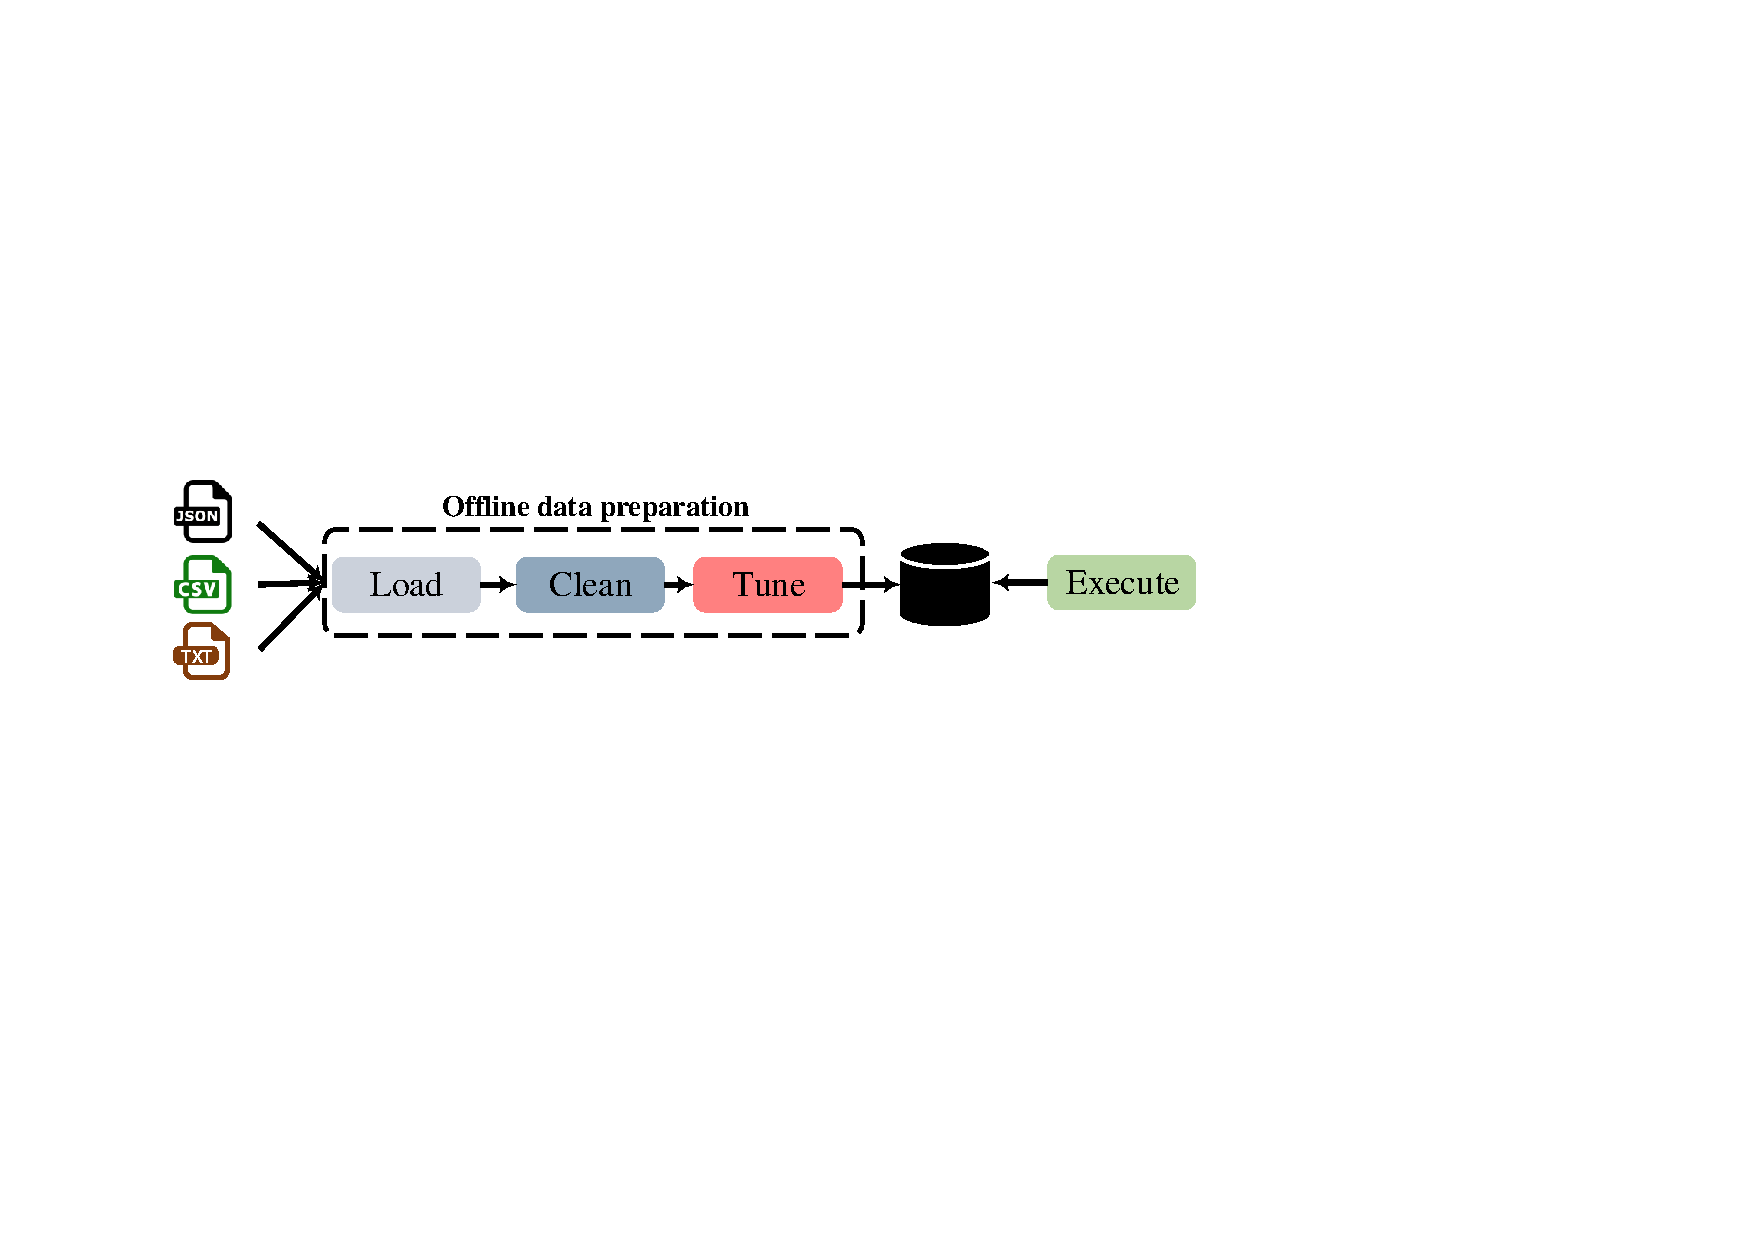
\includegraphics[page=1,width=0.7\columnwidth]{figs/data-preparation-offline}
%		\caption{Data Processing alternatives.}
		\caption{Data Processing pipeline.}
		\label{fig:alternatives}
	\end{center}
	\vspace{-2em}
\end{figure*}
%
\fref{fig:alternatives} presents the data pipeline of a 
state-of-the-art data analytics framework. The data to be analyzed is collected 
from a variety of sources, and might appear in various formats (e.g., XML, CSV, etc.). 
The multiple input formats are transformed into a single uniform format by loading
them into a DBMS. Then, to remove any inconsistencies cleaning operations are applied. Finally, 
a tuner builds access paths for 
efficient access. The final result is stored in a clean and tuned 
database, and is ready to receive query requests.

% re-cap and prepare for upcoming paragraphs
The preprocessing steps are exploratory and data-intensive, as they involve expensive operations, and highly depend on the data and the query workload. Data preparation tasks access the entire dataset multiple times: data loading results in copying and transforming the whole dataset into a common format. Cleaning tasks perform multiple passes over the data until they fix all the inconsistencies. Finally, to build indexes, an extra  traversal of the dataset is needed. Therefore, the increasing 
data volume limits the scalability of data preparation.
%
Furthermore,  the benefits of data preparation depend highly on the 
to-be executed workload. Data transformation and cleaning are only 
useful if the queries are data intensive and access the majority of 
data. Finally, tuning requires a priori knowledge of queries to decide 
upon the most efficient physical design.


\begin{wrapfigure}{L}{0.35\textwidth}
%		\centering
	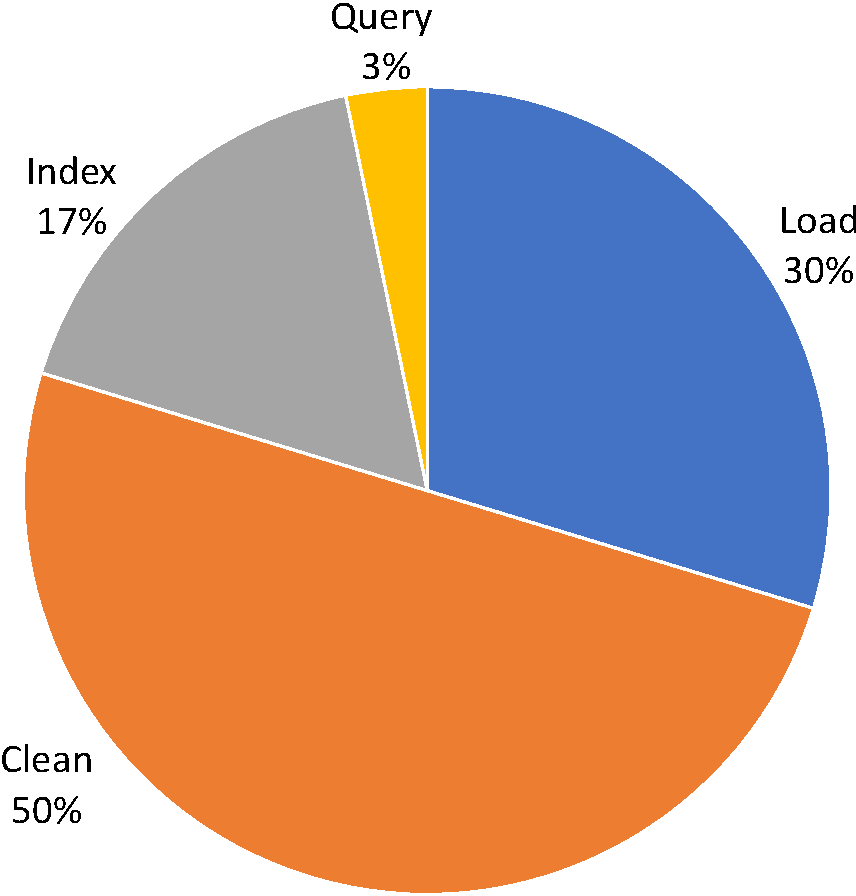
\includegraphics[width=0.34\columnwidth]{figs/breakdown_pie}	
	\caption{Cost of Data Preprocessing}
	\label{fig:preprocessing}
\end{wrapfigure}

% Tech problem 1: These are very expensive and take a very long time.
\Paragraph{Data preparation is time consuming} 
Due to the influx of data, data preparation becomes increasingly 
expensive. ~\fref{fig:preprocessing} demonstrates the breakdown of
the overall execution time of a typical data analysis scenario.
The breakdown corresponds to the time that a system requires to 
preprocess the data and execute a set of 10 queries. The execution 
time reported at 
each step is based on recent studies on loading, cleaning, and tuning 
\cite{buckley_new_2012,Olma2017a}.
Specifically, assuming an optimistic scenario in which data cleaning
corresponds to 50\% of the analysis time, then based on \cite{Olma2017a},
the rest 50\% 
is mostly spent on loading and tuning. The loading percentage may become even higher 
in the presence of non-relational data formats, such 
as XML, because a DBMS will have to flatten the dataset in order to 
load it. Query execution takes 3\% of the overall time. Therefore, 
data preparation incurs a significant overhead to data analysis.

% Insight 1: We don't need to do them on the whole data but only on 
%the parts that we care about.
Despite enterprises collecting and preparing 
increasingly larger amounts of data for analysis, often the effectively useful 
data is considerably smaller than the full 
dataset~\cite{scientific_data,Papadomanolakis2004}. 
The trend of exponential data growth due to intense data generation 
and data collection is expected to persist, however, recent studies 
of the data analysis workloads show that typically only a small 
subset of the data is relevant and ultimately used by analytical 
and/or exploratory workloads~\cite{Chen2012a}. 
Therefore, having to preprocess the whole dataset results in wasting
effort on data which are unnecessary for the actual analysis.
% Insight 2: Approximation
Furthermore, modern-day analytics, are increasingly tolerant to 
result imprecision. In many cases, precision to ``last decimal'' is 
redundant for a query answer. Quick approximation with some error 
guarantee is adequate to provide insights about the 
data~\cite{Cormode2012}.
Thus, using query approximation, one can execute analytical  queries  
over small samples of the dataset, and obtain approximate results 
within a few percents of the actual value \cite{Olma2019}.

\Paragraph{Ever Changing Workload}
Modern businesses and scientific applications require interactive 
data access, which is characterized by no or little a priori workload 
knowledge and constant workload shifting both in terms of projected 
attributes and selected ranges of the data.
% motivating example
For example, an electricity monitoring company continuously collects 
information about the current and aggregate energy consumption, and 
other sensor measurements such as temperature. To optimize 
consumption, the company performs predictive analytics over 
smart home datasets, looking for patterns that indicate energy 
request peaks and potential equipment downtime~\cite{IBM2012}. 
Analyses in this context start by identifying relevant 
measurements by using range queries and aggregations to identify 
areas of interests. The analysis focuses on specific data regions for 
a number of queries, but is likely to shift across the dataset to a 
different subset.
% we cannot predict what to prioritize and how to do this.
Due to the unpredictable nature of data analytics workloads, where 
queries may change depending on prior query results, applications
prepare all data for data access to avoid result inconsistencies. 
This preparation requires investment of time and resources into data 
that may be useless for the workload, thereby delaying data analysis.

\Paragraph{Adapt to Data and Workload}
% What do we propose as an approach: Adaptivity
To address the aforementioned shortcomings, we revisit the data processing
pipeline, and aim to streamline the process of extracting insights from data. 
We reduce 
the overall time of data analysis by introducing approaches which adapt
online to workload and dataset, which reduce the cost of each of the 
steps of data analysis from data collection to result.
Specifically, to reduce the cost of loading, we execute queries over 
raw data files \cite{Alagiannis2012a, 
Karpathiotakis2016,Karpathiotakis2015,Karpathiotakis2014}, to reduce 
the cost of data cleaning we piggy-back operations over query 
execution and we only sanitize data affected by the queries 
\cite{query_driven_cleaning}. Finally, to reduce the cost of tuning, 
we take advantage of data distribution as well as relaxed precision 
constraints of applications and adapt access paths online and as a
by-product of query execution to data and 
workload~\cite{Olma2017a,Olma2019}. 
\fref{fig:online-query-execution} demonstrates the revised data 
analysis process which weaves data preprocessing into query execution 
by adapting to the underlying data, as well as to the query workload.

% what is our design?
At the core of our approach lies \textit{in-situ} query processing, 
which allows the execution of declarative queries over external files 
without duplicating or ``locking'' data in a proprietary database 
format. 
% adapt to data formats
We extend \textit{in-situ} approaches 
\cite{Alagiannis2012a,Idreos2011} by treating any data format as a 
first-class citizen. To minimize query response times, we build a 
just-in-time query engine specialized for executing queries over 
multiple data formats. This approach removes the need for 
transforming and loading, while also offering low data access cost.
%
% adapt cleaning
To reduce the cost of data cleaning, we enhance query execution by 
injecting data cleaning operations inside the query plan. 
Specifically, we introduce a query answer relaxation technique which 
allows repairing erroneous tuples at query execution time. By 
relaxing the query answer, we ensure that the query returns all entities 
that may belong to the query result (e.g., no missing tuples).
%
% adapt access paths
Finally, similarly to data cleaning, building indexes over a 
dataset is becoming increasingly harder due to (i) shifting workloads 
and (ii) increasing data sizes which increase access path size as 
well.
The decision on what access paths to build depends on the expected 
workload, thus, traditional database systems assume knowledge of future 
queries. However, the shifting workload of modern data analytics can 
nullify investments towards indexing and other auxiliary data 
structures. Furthermore, access path size increases along with input 
data, thus, building precise access paths over the entire dataset 
limits the scalability of databases systems.
To address these issues, we adapt access paths to data 
distribution and precision requirements of the result. This enables 
building data structures specifically designed to take advantage of 
different data distributions and create data summaries requiring less 
storage space.

\begin{figure*}[t]
	\begin{center}
		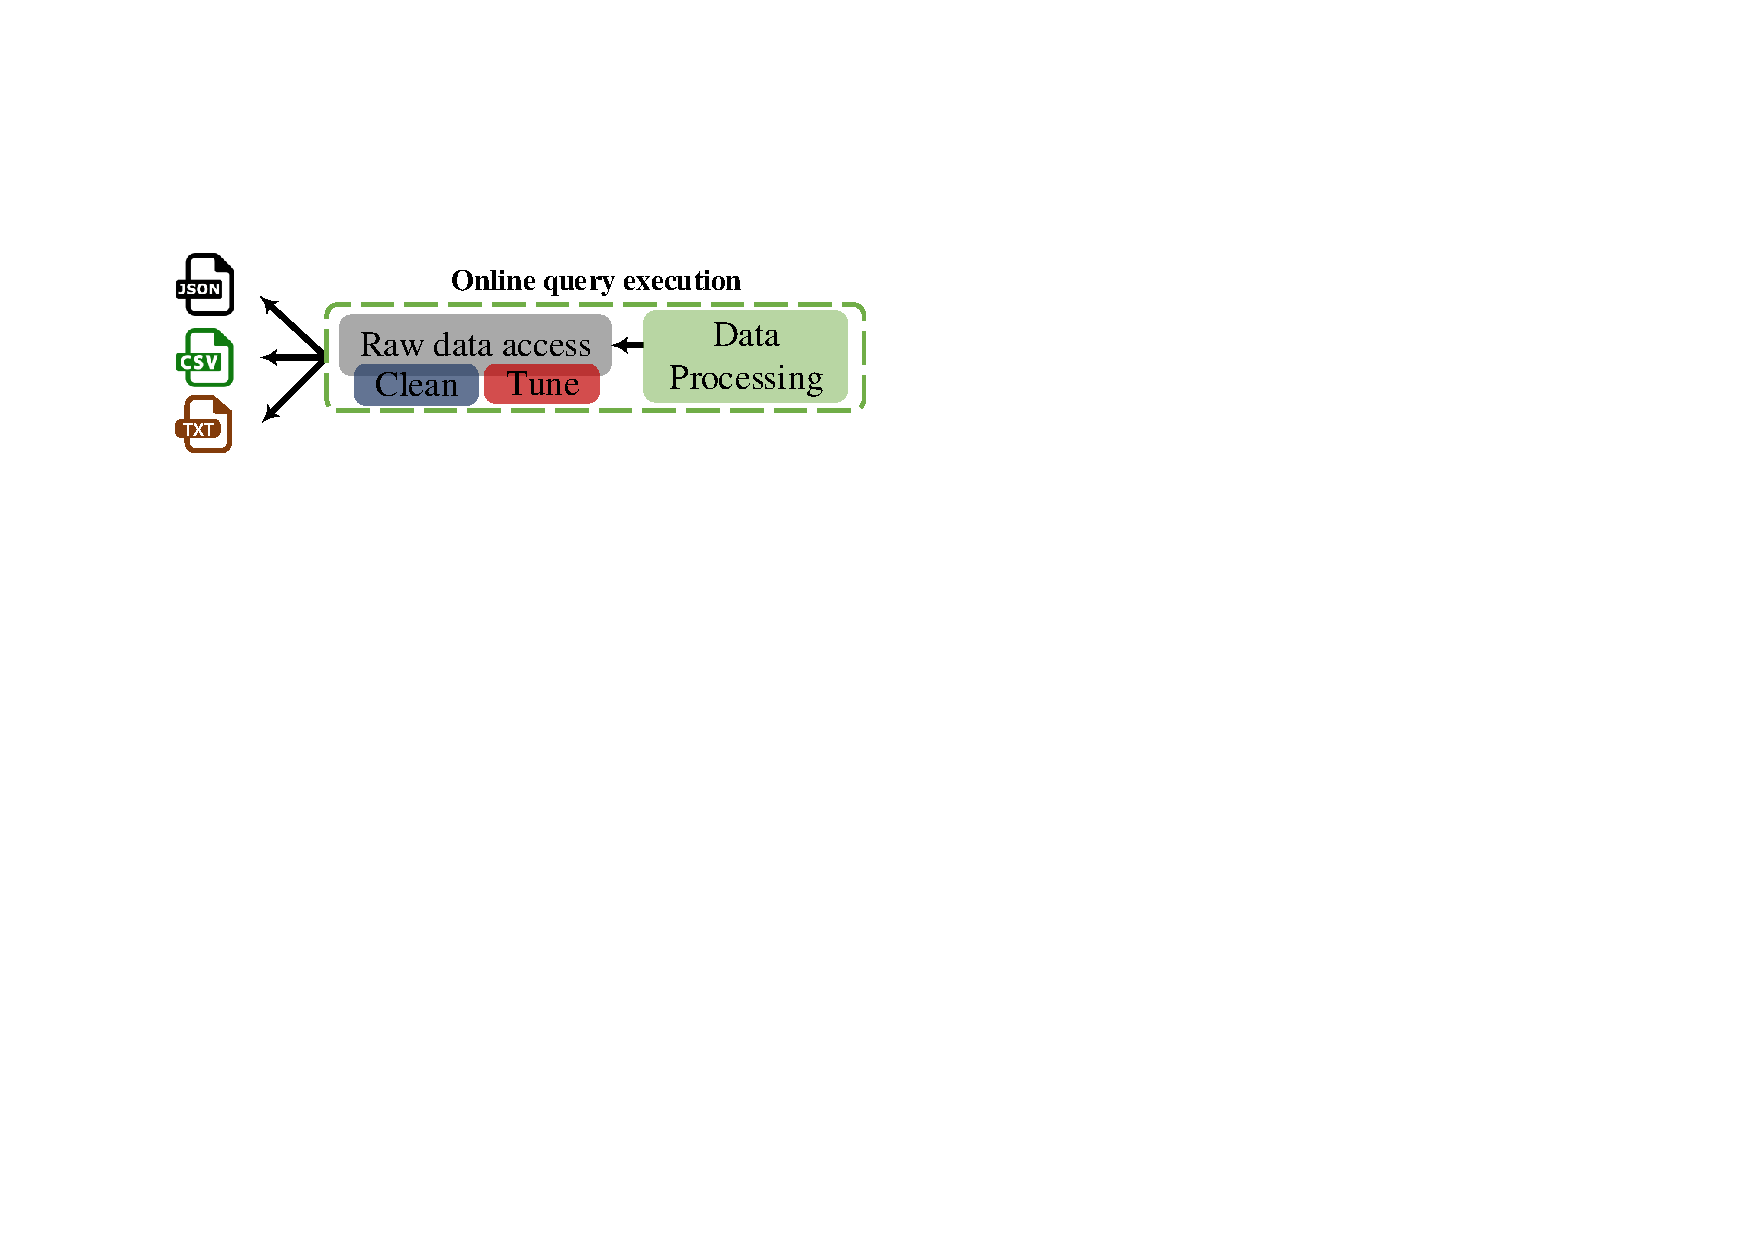
\includegraphics[page=1,width=0.5\columnwidth]{figs/query-execution-online}
		\caption{Integrating Cleaning and Tuning to Data Access.}
		\label{fig:online-query-execution}
	\end{center}
	\vspace{-2em}
\end{figure*}

In this paper we describe techniques that enable instant access to 
data irrespective of data format, and enable data cleaning and tuning 
without interrupting query execution. Each technique addresses a step 
in the preprocessing phase of data analysis, reducing the total 
data-to-insight time for users. Specifically, in~\sref{sec:proteus}, 
we describe the design behind our just-in-time query engine which 
enables efficient query execution despite data heterogeneity. 
In~\sref{sec:cleaning}, we demonstrate a novel approach to intertwine 
query execution with data cleaning through query answer relaxation. 
Our approach incrementally cleans only data that will be analyzed. 
In~\sref{sec:accesspaths}, we present our approach to adapt access 
paths online to data distribution and to precision requirements, as 
well as to available storage resources. Finally, 
in~\sref{sec:conclusion}, we conclude by highlighting techniques and 
related open problems for adaptive data management systems.
	%!TEX root=../bulletin.tex
\section{Adapting Data Access and Query Engine to Data Format}
\label{sec:proteus}

% introducing the two problems (expressing data generally enough and 
%running queries on multiple data formats)
Data analysis requires combining information from numerous 
heterogeneous datasets. For example, applications such as sensor data 
management and decision support based on web click-streams involve 
queries over data of varying models and formats. 
To support analysis workloads over heterogeneous datasets, 
practitioners are left with two alternatives: 
a) use a database engine that supports multiple operations 
\cite{onesize_fitsall}, %, but this approach  is expensive. Database 
%engines are typically generic and hard to 
%optimize for all cases. 
or b) execute their analysis over dedicated, specialized systems for each of their applications~\cite{xml_to_relational}. 
The first approach might hurt performance for scenarios involving 
non-relational data, but allows for extensive functionality and 
expressiveness. The second approach 
requires using multiple tools, as well as writing custom scripts to 
combine the results. Hence, performing analysis effortlessly and 
efficiently is challenging.

We present an approach that bridges the 
conflicting requirements for flexibility and performance when analyzing data of various formats. 
We achieve that by combining an optimizable query 
algebra, richer than the relational one, with on-demand adaptation 
techniques to eliminate numerous query execution overheads.

% algebra
\subsection{An Expressive Query Algebra}
To support queries over heterogeneous data, we need a query algebra that 
treats all supported data types as first-class citizens in terms of 
both expressive power and optimization capabilities.
Specifically, our approach is based on the monoid comprehension 
calculus~\cite{monoids}. A monoid is an algebraic construct term 
stemming from category theory which can be used to capture operations between both
primitive and collection data types. Therefore, monoids are a natural
fit for querying various data formats because they support operations over several data 
collections (e.g., bags, sets, lists, arrays) and arbitrary nestings 
of them. 
%

The monoid calculus provides the expressive power to manipulate different
data formats, and optimizes the resulting queries in a uniform way. First, the monoid
calculus allows transformations across data models by translating them
into operations over different types of collections, hence we can produce 
multiple types of output. The calculus is also expressive enough for 
other query languages to be mapped to it as syntactic sugar: For 
relational queries over flat data (e.g., binary and CSV files), our 
design supports SQL statements, which it translates to 
comprehensions. Similarly, for XML data, XQuery expressions can be
translated into our internal algebra.
%
Thus, monoid comprehensions allow for powerful manipulations of complex data 
as well as for queries over datasets 
containing hierarchies and nested collections (e.g., JSON arrays).
% step by step
% step 1

For each incoming query, the first step is mapping it into the internal language
that is based on monoid comprehensions. 
% re-write
Then, the resulting monoid comprehension is rewritten to an algebraic plan of the 
nested relational algebra~\cite{monoids}. This algebra resembles the 
relational algebra, with the difference that it allows more complex operators, which 
are applicable over hierarchical data. For example, apart from the
relational operators, such as selection and join, it provides
the unnest and outer unnest operators which ``unroll" a collection
field path that is nested within an object. Therefore, the
logical query plan allows for optimizations that combine the aforementioned operators.

The optimizer is responsible for performing the query rewriting and the conversion 
of a logical to a physical query plan. To apply the optimizations, the optimizer
takes into consideration both the existence of hierarchical data, as well as
that the queries might be complex, containing multiple nestings.
Therefore, the optimization involves a normalization algorithm \cite{monoids} 
which transforms the comprehension into a ``canonical'' form. The normalization 
also applies a series of optimization rewrites. Specifically, 
it applies filter pushdown and operator fusion. In addition, it
flattens multiple types of nested comprehensions. Thus, using the normalization
process, the comprehension is mapped to an expression that allows efficient
query execution.

The monoid comprehension calculus
is a rich model, and therefore incurs extra complexity. The more complex an algebra 
is, the harder it becomes to evaluate queries efficiently: Dealing 
with complex data leads to complex operators, sophisticated yet 
inefficient storage layouts, and costly pointer chasing during query 
evaluation. To overcome all previous limitations, we couple a broad 
algebra with on-demand customization.

% engine
\subsection{Query Engines On-Demand}
%The presented algebra allows combining data of heterogeneous models 
%and produces data-model-conscious query plans. 
%However, having a rich model and algebra incurs extra complexity.
%The more complex an algebra is in terms of expressive power, the 
%harder it becomes to evaluate queries efficiently: Dealing 
%with complex data leads to complex operators, sophisticated yet 
%inefficient storage layouts, and costly pointer chasing during query 
%evaluation. To overcome all previous limitations, we couple a broad 
%algebra with on-demand customization.

%
We couple this powerful query algebra with on-demand adaptation 
techniques to eliminate the query execution overheads stemming from
the complex operators. For analytical queries over flat (e.g., CSV) 
data, the system must behave as a relational system. 
Similarly, for hierarchical data, it must be as fast as a document store.
Specifically, our design is modular, with each of the modules using a 
code generation mechanism to customize the overall system across a 
different axis. 

%
First, to overcome the complexity of the broad algebra,we avoid the 
use of general-purpose abstract operators. Instead, we dynamically 
create an optimized engine implementation per query using code 
generation. Specifically, using code generation, we avoid the 
interpretation overhead by traversing the query plan only once and 
generating a custom implementation of every visited operator.  
Once all plan operators have been visited, the system can produce 
a hard-coded query engine implementation which is expressed in machine code.

%
To treat all supported data formats as native storage,  we 
customize the data access layer of the system based on the underlying 
data format while executing the query. Specifically, we mask the details of the underlying 
data values from the
query operators and the expression generators. To interpret data
values and generate code evaluating algebraic expressions, we use 
input plug-ins where each input plug-in is responsible for generating data 
access primitives for a specific file format. 


%
Finally, to utilize the storage that better fits the current workload, 
we materialize in-memory caches and treat them as an extra input. The 
shape of each cache is specified at query time, based on the format of
the data that the query accesses. 
We trigger cache creation i) implicitly, as a by-product of an 
operator's work, or ii) explicitly, by introducing caching operators 
in the query plan. Implicit caching exploits the fact that
some operators materialize their inputs: nest and join are
blocking and do not pipeline data. Explicit caching places buffering operators at any
point in the query plan. An explicit caching operator calls an output 
plug-in to populate a memory block with data. Then, it passes
control to its parent operator. Creating a cache adds an overhead to
the current query, but it can also benefit the overall query workload.

Our design combines i) an expressive query algebra which masks data 
heterogeneity with ii) on-demand customization mechanisms which produce a specialized
implementation per query. Based on this design, we build Proteus,
a query engine that natively supports different data formats, and specializes 
its entire architecture to each query and the data that it touches 
via code generation. Proteus also customizes
its caching component, specifying at query time how these caches
should be shaped to better fit the overall workload.

%Overall, the originally 
%distinct modules collapse into a unified, specialized query engine at 
%runtime. 
% shall I drop this?
%We validate our design by building Proteus, an analytical query 
%engine that queries heterogeneous datasets without converting them to 
%a homogeneous form. Proteus couples a general query interface with 
%the execution times of a system that has been specialized for a 
%specific query, data, and workload instance. Proteus currently 
%supports CSV, JSON, and relational binary data. Its modularity makes 
%it extensible; adding support for more formats is straightforward.
	%!TEX root=../bulletin.tex
\section{Cleaning Data while Discovering Insights}
\label{sec:cleaning}

%The process of gathering, storing, and integrating diverse 
%datasets introduces several inaccuracies in the data:
%Analysts spend 50\%-80\% 
%of their time preparing dirty data before it can be used for information 
%extraction \cite{buckley_new_2012}. 
%Therefore, data cleaning is a major hurdle for data analysis.
%
%Data scientists apply cleaning tasks in an iterative fashion to identify and
%fix inconsistencies until they obtain a clean version of the dataset that
%is ready for the analysis they need to perform. Therefore, data
%cleaning is subjective and time-consuming.

Data cleaning is an interactive and exploratory process which involves expensive operations. 
Error detection requires multiple pairwise comparisons to check the satisfiability of the given constraints \cite{cleanm}.
Data repairing adds an extra overhead since it requires multiple iterations in order to assign candidate values to the
erroneous cells until all constraints are satisfied \cite{nadeef,data_quality,bigdansing,Stonebraker_datacuration}. 
At the same time, data cleaning depends on the analysis that users perform;
data scientists detect inconsistencies, and determine the required data cleaning operations 
while exploring through the dataset \cite{eda}. 
Therefore, the usage of offline data cleaning approaches requires long running times in order to discover and fix the discrepancies that might affect data analysis.

To address the efficiency problem, as well as the subjective nature of data cleaning, there 
is need for a data cleaning approach which
is weaved into the data analysis process, and which also applies data cleaning on-demand. 
Integrating data cleaning with data analysis efficiently supports exploratory data analysis \cite{exploratory_analysis}, and ad-hoc data analysis applications \cite{transform-by-ex} 
by reducing the number and the cost of iterations required in order to extract insights out of dirty data.
In addition, by cleaning data on the fly, one only loads and cleans necessary data thereby minimizing wasted effort whenever only a subset of data is analyzed.

%%By coupling data cleaning with data analysis, we reduce the data cleaning cost by focusing only on 
%%the interesting part of the dataset, that is, the part that the user accesses through the exploratory analysis process.
%To provide correct answers over dirty data, we employ query answer relaxation \cite{online_queryrelax, queryrelax_incomplete}. 
%Query relaxation has been used successfully to address the problem of queries returning no results, 
%or to facilitate query processing over incomplete databases. We define and employ a novel query relaxation technique in the context of 
%dirty data, in order to enhance the query answer with the appropriate information from the dataset that allows the
%detection of violations of integrity constraints.Then, given the detected errors, we propose candidate fixes by providing
%probabilistic answers \cite{probabilistic_dbs}.
%After the execution of each query, we isolate the changes made in the dataset and we apply the delta to the original dataset.
%Thus, we incrementally obtain a clean instance of the dataset by adding an overhead to each query. In addition, we build a
%cost model which decides between incremental cleaning and full cleaning by taking into consideration the type of
%queries, the number of violations of the dataset, and the accuracy of the resulting answer. 
%%We validate our approach by building Daisy, a distributed incremental cleaning framework over Spark \cite{spark}.

We intermingle cleaning integrity constraint violations \cite{dependencies} with exploratory data analysis, in order to gradually clean the dataset. 
Specifically, given a query and a dirty dataset, we use two levels of processing to correctly execute the query
by taking into consideration the existence of inconsistencies in the underlying dataset. In the first level, we map the query to a logical plan 
which comprises both query and cleaning operators. The logical plan
takes into consideration
the type of the query (e.g, Select Project, Join), and the constraints that the dataset needs to satisfy in order to optimally place the cleaning operators inside the query plan. 
Then, in the second level, the logical plan is executed by applying the cleaning tasks that are needed. To execute the plan, we employ a query answer relaxation technique, which enhances the answer of the query with
extra information from the dataset in order to 
detect violations based on the output of each query operator that is affected by a constraint. 
Then, given the detected violations, we transform the query answer into a probabilistic
answer by replacing each erroneous value with the set of values that represent candidate fixes for that value.
In addition, we accompany each candidate value with the corresponding probability of being the correct value of the erroneous cell. 
After cleaning each query answer, the system extracts the changes made to the erroneous
tuples, and updates the original dataset accordingly. By applying the changes after each
query, we can gradually clean the dataset.

\subsection{Logical-level Optimizations} 
In the first stage, the system translates the query into a logical plan involving query and
cleaning operators. The cleaning operators are update operators which either operate over the underlying 
dataset, or over the condition that exists below them in the query plan.
To place the cleaning operators, the system determines whether it is more efficient and/or accurate to integrate the 
query with the cleaning task, and partially clean the dataset, or to fully clean the dataset before executing the query. To decide on the cleaning strategy, 
we employ a cost model which exploits statistics regarding the type and frequency of the violations.
To optimally place the cleaning operators, the system examines: a) the approximate number of violations that exist in the dataset, and 
b) how the query operators overlap with the erroneous attributes. Thus, the statistics provide an estimate of the overhead that the cleaning task adds to each query, and determine the optimal placement of the cleaning operations.


At the logical plan level, we apply a set of optimizations by pruning unnecessary cleaning checks,
and unnecessary query operators. To apply the optimizations, we
analyze how the input constraints that must hold in the dataset affect the query result.
For example, it is redundant to apply a cleaning task in the case of a query that contains a filter condition over a clean attribute.
Therefore, the logical plan will select the optimal execution strategy of the queries given the cleaning tasks that need to be applied.

\subsection{Relaxed query execution}
In the final stage, the system executes the optimized logical plan, and computes
a correct query answer by applying the cleaning tasks at query execution. 
Regardless of the type of query, we need to enhance the query answer with extra tuples from the dataset to allow the detection and repairing of errors.
Executing queries over dirty data might result in wrong query answers \cite{incomplete_dbs}; a tuple might erroneously satisfy a query and appear in the query answer
due to a dirty value, or similarly, it might be missing from the query answer due to a dirty value. 

To provide correct answers over dirty data, we employ query answer relaxation \cite{online_queryrelax, queryrelax_incomplete}. 
Query relaxation has been used successfully to address the problem of queries returning no results, 
or to facilitate query processing over incomplete databases. We define and employ a novel query answer relaxation technique in the context of querying
dirty data, which enhances the query answer with extra tuples from the dataset that allow the
detection of violations of integrity constraints. Then, given the detected errors, we propose candidate fixes by providing
probabilistic answers \cite{probabilistic_dbs}. The probabilities are computed based on the frequency that each candidate value appears - other schemes to infer the probabilities are also applicable.
The purpose of the query answer relaxation mechanism is to enhance the query answer with the required information from the dataset, in order to allow correct answers to the queries. 

To capture errors in query results, we first compute the dirty query answer, and then relax it by bringing extra tuples from the dataset; the extra tuples, together with the tuples of the query answer represent the candidates for satisfying the query. The set of extra tuples consist of tuples which are similar to the ones belonging to the query answer; the similarity depends on the correlation that the tuples have with respect to the integrity constraints that hold in the dataset \cite{scare}. 
After enhancing the query answer with the extra tuples, the cleaning process detects for violations and computes the set of
candidate values for each erroneous cell together with their probabilities. 

By integrating data cleaning with query execution using the aforementioned two-level process, we minimize the cost of data preparation; we efficiently clean only the part of the dataset that is accessed by the queries. In addition, by providing
probabilistic answers for the erroneous entities, we reduce human effort, since users can select the correct values among the set of candidate values over the answers of the queries.

%In a nutshell, based on the 
%logical plan, when the system checks a condition (e.g., \textit{select} or \textit{join} predicate), it enhances the result of the operator with extra tuples from the dataset in order
%to allow the error detection and data repairing operations.  



	%!TEX root=../bulletin.tex
\section{Adapting Data Access Paths to Workload and Resources}
\label{sec:accesspaths}

Apart from loading and cleaning decisions,
as data-centric applications become more complex, users face new 
challenges when exploring data, which are magnified with the 
ever-increasing data volumes. %Database systems must embrace 
%adaptivity and provide query processing approaches 
%that enable efficient execution of shifting workloads. 
Data access methods have to dynamically adapt to evolving workloads 
and take advantage of relaxed accuracy requirements. Furthermore, 
query processing systems must be knowledgeable of the available 
resources and maximize resource utilization thereby reduce waste. 
To address the variety of workloads we design different adaptive 
access path selection approaches depending on application precision 
requirements.

\Paragraph{Adaptive indexing over raw data} To achieve 
efficient data access for applications requiring precise results 
despite dynamic workloads we propose adaptive indexing for in-situ 
query processing. We use state-of-the-art in-situ query 
processing approaches to minimize data-to-query time. We 
introduce a fine-grained logical partitioning scheme and combine it 
with a lightweight indexing strategy to provide near-optimal raw data 
access with minimal overhead in terms of execution time and memory
footprint. To reduce the index selection overhead we propose an 
adaptive technique for on-the-fly partition and index selection using 
an online randomized algorithm.

\Paragraph{Adapt access paths to approximation}
Apart from adapting to data distribution, we need to enable scaling 
of access paths despite ever-increasing datasets. We take advantage 
of the relaxed precision requirements posed by data scientists who 
tolerate imprecise answers for better query 
performance~\cite{Cormode2012}. 
Existing approaches~\cite{Agarwal2013,Chaudhuri2001b}, either require 
full a priori knowledge of the workload to generate the required 
approximate data structures or improve performance through minimizing 
data access at query time. We design and demonstrate an adaptive 
approach which generates synopses (summaries of the data, such as 
samples, sketches, and histograms) as a by-product of query execution 
and re-uses them for subsequent queries. It dynamically decides upon 
synopsis materialization and maintenance while being robust to 
workload and storage budget changes. To support interactive query 
performance for ever increasing datasets and dynamic exploratory 
workloads there is need for relaxed precision guarantees which enable 
the use of approximate data structures and reduce the size of stored 
and processed data.

These aforementioned observations serve as a platform to show the 
following key insights:
i) Taking advantage of data characteristics in files can complement 
in-situ query processing approaches by building data distribution 
conscious access paths. Data properties such as ordering or 
clustering enable the construction of access paths spanning subsets of
a dataset thereby reducing the cost of tuning and storage, while minimizing 
data access costs and further reducing the data-to-insight time.
ii) Ever-increasing datasets make precise access paths prohibitively 
expensive to build and store. Similarly, using data synopses as a 
drop-in replacement for indexes limits their benefits. On the 
contrary, integrating synopses as a first-class citizen in query
optimization and materializing synopses during query execution and 
re-using them across queries improves scalability and reduces 
preprocessing.
iii) Static tuning decisions can be suboptimal in the presence of 
shifting exploratory workloads. On the other hand, adapting access 
paths online, according to the workload while adhering to accuracy 
requirements is key to provide high query performance in the
presence of workload changes.

\subsection{Adaptive indexing over Raw data files}

Executing queries over raw data files, despite reducing cost through 
avoiding the initial data loading step, it enables the access of data 
files by multiple applications thus it prohibits the physical 
manipulation of data files. 
Building efficient data access paths requires physical 
re-organization of files to reduce random accesses during query 
execution. To overcome this constraint we propose an online 
partitioning and indexing tuner for in-situ query processing which 
when plugged into a raw data query engine, offers fast queries over 
raw data files. The tuner reduces data access cost by: 
i) logically partitioning a raw dataset to virtually break it
into smaller manageable chunks without physical restructuring, and 
ii) choosing appropriate indexing strategies over each logical 
partition to provide efficient data access. 
The tuner dynamically adapts the partitioning and indexing scheme as a 
by-product  of query execution.
It continuously collects information regarding the values and access 
frequency of queried attributes at runtime. Based on this 
information, it uses a randomized online algorithm to define the 
logical partitions. For each logical partition, the tuner estimates 
the cost-benefit of building partition-local index structures 
considering both approximate membership indexing
(i.e., Bloom filters and zone maps) and full indexing (i.e., bitmaps 
and B + trees). By allowing fine-grained indexing decisions our 
proposal makes the decision of the index shape at the level of each 
partition rather than the overall relation. This has two positive 
side-effects. First, there is no costly investment for indexing that 
might prove unnecessary. Second, any indexing effort is tailored to 
the needs of data accesses on the corresponding range of the dataset.

\subsection{Adapting to Relaxed Precision}

State-of-the-art AQP engines are classified into two categories,
depending on the assumptions they make about the query workload.
\emph{Offline AQP} engines (e.g. BlinkDB~\cite{Agarwal2013} and 
STRAT~\cite{Chaudhuri2001b}) target applications where the query 
workload is known a priori, e.g., aggregate dashboards that compute 
summaries over a few fixed columns. Offline AQP engines analyse the 
expected workload to identify the optimal set of synopses that should 
be generated to provide fast responses to the queries at hand, 
subject to a predefined storage budget and error tolerance 
specification. Since this analysis is time-consuming, both due to the 
computational complexity of the analysis task, as well as the I/O 
overhead in generating the synopses, AQP engines perform the analysis 
offline, each time the query workload or the storage budget changes.
Offline AQP engines substantially improve query execution time 
under predictable query workloads, however their need for a priori knowledge 
of the queries makes them unsuitable for unpredictable workloads. 
%
To address unpredictable workloads \emph{online AQP} techniques 
introduce approximation at query runtime. State-of-the-art online AQP 
engines achieve this by introducing samplers during query execution. 
By reducing the input tuples, samplers improve performance of the 
operators higher in the query plan. In this way, online AQP 
techniques can boost unknown query workloads. However, query-time 
sampling is limited in the scope of a single query, as the generated 
samples are not constructed with the purpose of reuse across queries 
-- they are specific to the query, and are not saved. Thus, online 
AQP engines offer substantially constrained performance gains 
compared to their offline counterparts for predictable workloads.

In summary, all state-of-the-art AQP engines sacrifice either 
generality or performance, as they make 
static, design-time decisions based on a fixed set of assumptions 
about the query workload and resources. 
However, modern data analytics workloads are complex, far 
from homogeneous, and often contains a mix of queries that vary 
widely with respect to the degree of 
approximability~\cite{Agarwal2013}. 

We design a self-tuning, adaptive, online AQP engine. Our design 
builds upon ideas from (adaptive) database systems, such as 
intermediate result materialization, query subsumption, materialized 
view tuning and index tuning, and adapts these in the context of AQP, 
while also enabling a combination and extension of the benefits of both offline 
and online approximation engines. 
%
We extend the ideas of online AQP by injecting approximation 
operators in the query plan, and enabling a broad range of queries over 
unpredictable workloads.
By performing online materialization of synopses as a byproduct of 
query execution, we provide performance on-par with offline AQP 
engines under predictable workloads, yet without an expensive offline 
preparation phase. 
%
The main components of our system are the enhanced optimizer which enables the 
use of approximate operators and matches existing synopses, and the 
online tuner which decides on the materialization of intermediate results.

\Paragraph{Integrating approximation to optimizer} Our system extends 
a query optimizer with just-in-time approximation capabilities. 
% inject synopsis operators
The optimizer injects synopses operators into the query plan before 
every aggregation. Intuitively, this represents the potential to 
approximate at that location. 
% transformation
Subsequently, by using transformation rules, it pushes the synopses 
operators closer to the raw input. The alternatives generated by 
rules have no worse accuracy but can have better performance. 
% costing
The optimizer calculates the cost of each plan using data statistics 
to decide a plan that adheres to user accuracy requirements and 
improves performance.
%
Based on the generated query plans, the optimizer compares whether 
any of the already materialized synopses may be re-used. To be 
re-used a synopsis must (i) satisfy the accuracy guarantees  
requirements, and (ii) subsume the required set of data.
%
If no existing synopses are candidates for re-use, the optimizer 
interacts with the online tuner to decide whether to materialize 
intermediate results.

\Paragraph{Online Tuner}
The optimizer feeds every prospective approximate plan to the online 
tuner which stores execution metadata considering historical plans 
(e.g., appearance frequency, execution cost).
%
Based on the historical plans, the tuner decides whether to introduce 
a materializer operator to generate a summary. The tuner's
decisions are driven by a cost:utility model, which leads to a 
formalization of the task as an optimization challenge. As the 
optimizer already ensures the precision of the query results, the 
decisions made by the tuner affect solely query performance, and not 
the required accuracy.
%
Finally, the tuner keeps track of the available storage budget and 
decides on storage location and replication for a materialized 
sub-plan. The tuner based on the available storage and the 
cost:benefit model decides whether and which synopses to be stored or 
evicted.

By using approximate query processing one allows for low latency in return for 
relaxed precision. However, the ever-increasing data sizes introduce 
challenges to such systems. Specifically, offine approximation 
approaches in order to offer low response time, they require long 
pre-processing, full future workload knowledge and have high storage 
requirements. On the other hand, online approximation approaches 
although have no preprocessing, storage requirements and are
workload-agnostic they have small performance gains. Our approach 
adaptively combines the two approaches and trades precision and 
storage for performance at runtime offering the best of both worlds.
	%!TEX root=../bulletin.tex
\section{Related Work}
\label{sec:related}

Our philosophy has been inspired by the omnipresent work on minimizing data-to-insight time.
In-situ processing approaches, such as the work by Idreos et al. \cite{Idreos2011a} propose adaptive and incremental loading
techniques in order to eliminate the preparation phase before query execution. NoDB \cite{Alagiannis2015} advances this idea by making raw files first-class citizens. NoDB introduces data structures to adaptively index and cache raw files, tightly integrates adaptive loads, while implementing in-situ access into a modern DBMS. 
In the context of processing heterogeneous raw data,
Spark and Hadoop-based systems \cite{apache_drill,spark} operate over raw data, while also supporting heterogeneous data formats.
RAW \cite{Karpathiotakis2014} allows queries over heterogeneous raw files using code generation.
ViDa~\cite{Karpathiotakis2015} envisions effortlessly abstracting data out of its form and manipulating it regardless of its structure, in a uniform way.

Work on reducing the data cleaning cost by automating and optimizing common cleaning tasks significantly reduces human effort and minimizes the preprocessing cost. BigDansing \cite{bigdansing} is a scale-out
data cleaning system which addresses performance, and ease-of-use issues in the presence of duplicates and integrity constraint violations.
Tamr, the commercial version of Data Tamer \cite{Stonebraker_datacuration}, focuses on duplicate elimination
by employing blocking and classification techniques in order to efficiently detect and eliminate duplicate pairs.
In the context of adaptive and ad-hoc cleaning QuERy \cite{quERy} intermingles duplicate elimination with Select Project, and Join queries in order to clean only the data that is useful for the queries.
Transform-Data-by-Example \cite{transform-by-ex} addresses the problem of allowing on-the-fly transformations - a crucial part of data preparation.

Work on adaptive tuning focuses on incrementally refining indexes 
while processing queries. Database Cracking approaches 
\cite{Idreos2011} operate over column-stores and incrementally sort 
the index column according to the incoming workload, thus reducing 
memory access. COLT \cite{Schnaitter2006} continuously monitors the 
workload and periodically creates new indexes and/or drops unused 
ones by adding an overhead to each query.

A plethora of research topics on approximate query processing is also relevant to our work. Offline sampling strategies \cite{Agarwal2013,Chaudhuri2001b} focus on computing the best set of uniform and stratified samples given a storage budget by 
assuming some a priori knowledge of the workload. Online sampling approaches such as Quickr \cite{quickr} take samples during
query execution by injecting samplers inside the query plan.

	
	%!TEX root=../bulletin.tex
\section{Summary and Next Steps}
\label{sec:conclusion}

The constantly changing needs for efficient data analytics combined 
with the ever growing datasets, require  a system design which is 
flexible, dynamic and embraces adaptivity. We present techniques 
which streamline processes that constitute bottlenecks in data 
analysis and reduce the overall data-to-insight time. To remove data 
loading, we introduce a system that adapts to data heterogeneity and 
enables queries on variety of data formats. To reduce data cleaning 
overheads, we overlap cleaning operations with query execution and 
finally, we introduce physical tuning approaches which take advantage 
of data distribution as well as the reduced precision requirements of 
modern analytics applications.
		
%\bibliographystyle{abbrv}
%\bibliography{bibliography/library}
	\begin{thebibliography}{10}
	\itemsep=1pt
	\begin{small}
	\bibitem{apache_drill}
Apache drill.
\newblock \url{https://drill.apache.org/}.

\bibitem{Agarwal2013}
S.~Agarwal, B.~Mozafari, A.~Panda, H.~Milner, S.~Madden, and I.~Stoica.
\newblock {BlinkDB: Queries with Bounded Errors and Bounded Response Times on
  Very Large Data}.
\newblock In {\em Proceedings of the ACM European Conference on Computer
  Systems (EuroSys)}, pages 29--42, 2013.

\bibitem{Agrawal2004}
S.~Agrawal, S.~Chaudhuri, L.~Koll{\'{a}}r, A.~P. Marathe, V.~R. Narasayya, and
  M.~Syamala.
\newblock {Database Tuning Advisor for Microsoft SQL Server 2005}.
\newblock In {\em Proceedings of the International Conference on Very Large
  Data Bases (VLDB)}, pages 1110--1121, 2004.

\bibitem{scientific_data}
A.~Ailamaki, V.~Kantere, and D.~Dash.
\newblock Managing scientific data.
\newblock {\em Communications of the ACM}, 53, 06 2010.

\bibitem{Alagiannis2012a}
I.~Alagiannis, R.~Borovica, M.~Branco, S.~Idreos, and A.~Ailamaki.
\newblock {NoDB: Efficient Query Execution on Raw Data Files}.
\newblock In {\em Proceedings of the ACM SIGMOD International Conference on
  Management of Data}, pages 241--252, 2012.

\bibitem{Alagiannis2015}
I.~Alagiannis, R.~Borovica-Gajic, M.~Branco, S.~Idreos, and A.~Ailamaki.
\newblock {NoDB: Efficient Query Execution on Raw Data Files}.
\newblock {\em Communications of the ACM}, 58(12):112--121, 2015.

\bibitem{quERy}
H.~Altwaijry, S.~Mehrotra, and D.~V. Kalashnikov.
\newblock {QuERy: A Framework for Integrating Entity Resolution with Query
  Processing}.
\newblock {\em {PVLDB}}, 9(3), 2015.

\bibitem{Chaudhuri2001b}
S.~Chaudhuri, G.~Das, and V.~Narasayya.
\newblock {A Robust, Optimization-based Approach for Approximate Answering of
  Aggregate Queries}.
\newblock In {\em Proceedings of the ACM SIGMOD International Conference on
  Management of Data}, pages 295--306, 2001.

\bibitem{Chaudhuri1997}
S.~Chaudhuri and V.~R. Narasayya.
\newblock {An Efficient Cost-Driven Index Selection Tool for Microsoft SQL
  Server}.
\newblock In {\em Proceedings of the International Conference on Very Large
  Data Bases (VLDB)}, pages 146--155, 1997.

\bibitem{Chen2012a}
Y.~Chen, S.~Alspaugh, and R.~H. Katz.
\newblock {Interactive Analytical Processing in Big Data Systems: A
  Cross-Industry Study of MapReduce Workloads}.
\newblock {\em Proceedings of the VLDB Endowment}, 5(12):1802--1813, 2012.

\bibitem{Cormode2012}
G.~Cormode, M.~N. Garofalakis, P.~J. Haas, and C.~Jermaine.
\newblock {Synopses for Massive Data: Samples, Histograms, Wavelets, Sketches}.
\newblock {\em Foundations and Trends in Databases}, 4(1-3):1--294, 2012.

\bibitem{nadeef}
M.~Dallachiesa, A.~Ebaid, A.~Eldawy, A.~Elmagarmid, I.~F. Ilyas, M.~Ouzzani,
  and N.~Tang.
\newblock {NADEEF: A Commodity Data Cleaning System}.
\newblock In {\em {SIGMOD}}, 2013.

\bibitem{exploratory_analysis}
T.~Dasu and T.~Johnson.
\newblock {\em Exploratory Data Mining and Data Cleaning}.
\newblock John Wiley \& Sons, Inc., New York, NY, USA, 1 edition, 2003.

\bibitem{dependencies}
W.~Fan.
\newblock Dependencies revisited for improving data quality.
\newblock In {\em {PODS}}, 2008.

\bibitem{data_quality}
W.~Fan.
\newblock Data quality: From theory to practice.
\newblock {\em SIGMOD Rec.}, 44(3):7--18, Dec. 2015.

\bibitem{monoids}
L.~Fegaras and D.~Maier.
\newblock {Optimizing Object Queries Using an Effective Calculus}.
\newblock {\em TODS}, 25(4):457--516, Dec. 2000.

\bibitem{query_driven_cleaning}
S.~Giannakopoulou.
\newblock Query-driven data cleaning for exploratory queries.
\newblock In {\em {CIDR} 2019, 9th Biennial Conference on Innovative Data
  Systems Research, Asilomar, CA, USA, January 13-16, 2019, Online
  Proceedings}, 2019.

\bibitem{cleanm}
S.~Giannakopoulou, M.~Karpathiotakis, B.~Gaidioz, and A.~Ailamaki.
\newblock Cleanm: An optimizable query language for unified scale-out data
  cleaning.
\newblock {\em Proc. VLDB Endow.}, 10(11):1466--1477, Aug. 2017.

\bibitem{incomplete_dbs}
P.~Guagliardo and L.~Libkin.
\newblock Making sql queries correct on incomplete databases: A feasibility
  study.
\newblock In {\em Proceedings of the 35th ACM SIGMOD-SIGACT-SIGAI Symposium on
  Principles of Database Systems}, PODS '16, pages 211--223, New York, NY, USA,
  2016. ACM.

\bibitem{transform-by-ex}
Y.~He, K.~Ganjam, K.~Lee, Y.~Wang, V.~Narasayya, S.~Chaudhuri, X.~Chu, and
  Y.~Zheng.
\newblock Transform-data-by-example (tde): Extensible data transformation in
  excel.
\newblock In {\em Proceedings of the 2018 International Conference on
  Management of Data}, SIGMOD '18, pages 1785--1788, New York, NY, USA, 2018.
  ACM.

\bibitem{IBM2012}
IBM.
\newblock {Managing big data for smart grids and smart meters}.
\newblock {\em IBM White Paper}, 2012.

\bibitem{Idreos2011a}
S.~Idreos, I.~Alagiannis, R.~Johnson, and A.~Ailamaki.
\newblock {Here are my Data Files. Here are my Queries. Where are my Results?}
\newblock In {\em Proceedings of the Biennial Conference on Innovative Data
  Systems Research (CIDR)}, pages 57--68, 2011.

\bibitem{Idreos2011}
S.~Idreos, S.~Manegold, H.~Kuno, and G.~Graefe.
\newblock {Merging What's Cracked, Cracking What's Merged: Adaptive Indexing in
  Main-Memory Column-Stores}.
\newblock {\em Proceedings of the VLDB Endowment}, 4(9):586--597, 2011.

\bibitem{quickr}
S.~Kandula, A.~Shanbhag, A.~Vitorovic, M.~Olma, R.~Grandl, S.~Chaudhuri, and
  B.~Ding.
\newblock {Quickr: Lazily Approximating Complex AdHoc Queries in BigData
  Clusters}.
\newblock In {\em SIGMOD}, 2016.

\bibitem{Karpathiotakis2016}
M.~Karpathiotakis, I.~Alagiannis, and A.~Ailamaki.
\newblock {Fast Queries Over Heterogeneous Data Through Engine Customization}.
\newblock {\em Proceedings of the VLDB Endowment}, 9(12):972--983, 2016.

\bibitem{Karpathiotakis2015}
M.~Karpathiotakis, I.~Alagiannis, T.~Heinis, M.~Branco, and A.~Ailamaki.
\newblock {Just-In-Time Data Virtualization: Lightweight Data Management with
  ViDa}.
\newblock In {\em Proceedings of the Biennial Conference on Innovative Data
  Systems Research (CIDR)}, 2015.

\bibitem{Karpathiotakis2014}
M.~Karpathiotakis, M.~Branco, I.~Alagiannis, and A.~Ailamaki.
\newblock {Adaptive Query Processing on RAW Data}.
\newblock {\em Proceedings of the VLDB Endowment}, 7(12):1119--1130, 2014.

\bibitem{bigdansing}
Z.~Khayyat, I.~F. Ilyas, A.~Jindal, S.~Madden, M.~Ouzzani, P.~Papotti, J.-A.
  Quian{\'e}-Ruiz, N.~Tang, and S.~Yin.
\newblock {BigDansing: A System for Big Data Cleansing}.
\newblock In {\em {SIGMOD}}, 2015.

\bibitem{buckley_new_2012}
S.~Lohr.
\newblock {For Big-Data Scientists, 'Janitor Work' Is Key Hurdle to Insights,
  The New York Times}, 2014.

\bibitem{online_queryrelax}
I.~Muslea and T.~J. Lee.
\newblock Online query relaxation via bayesian causal structures discovery.
\newblock In {\em AAAI}, 2005.

\bibitem{Olma2017a}
M.~Olma, M.~Karpathiotakis, I.~Alagiannis, M.~Athanassoulis, and A.~Ailamaki.
\newblock {Slalom: Coasting Through Raw Data via Adaptive Partitioning and
  Indexing}.
\newblock {\em Proceedings of the VLDB Endowment}, 10(10):1106--1117, 2017.

\bibitem{Olma2019}
M.~Olma, O.~Papapetrou, R.~Appuswamy, and A.~Ailamaki.
\newblock {Taster: Self-Tuning, Elastic and Online Approximate Query
  Processing}.
\newblock In {\em Proceedings of the IEEE International Conference on Data
  Engineering (ICDE)}, 2019.

\bibitem{Papadomanolakis2004}
S.~Papadomanolakis and A.~Ailamaki.
\newblock {AutoPart: Automating Schema Design for Large Scientific Databases
  Using Data Partitioning}.
\newblock In {\em Proceedings of the International Conference on Scientific and
  Statistical Database Management (SSDBM)}, page 383, 2004.

\bibitem{Schnaitter2006}
K.~Schnaitter, S.~Abiteboul, T.~Milo, and N.~Polyzotis.
\newblock {COLT: Continuous On-Line Database Tuning}.
\newblock In {\em Proceedings of the ACM SIGMOD International Conference on
  Management of Data}, pages 793--795, 2006.

\bibitem{xml_to_relational}
J.~Shanmugasundaram, K.~Tufte, C.~Zhang, G.~He, D.~J. DeWitt, and J.~F.
  Naughton.
\newblock Relational databases for querying xml documents: Limitations and
  opportunities.
\newblock In {\em Proceedings of the 25th International Conference on Very
  Large Data Bases}, VLDB '99, pages 302--314, San Francisco, CA, USA, 1999.
  Morgan Kaufmann Publishers Inc.

\bibitem{queryrelax_incomplete}
S.~Shen.
\newblock Database relaxation: An approach to query processing in incomplete
  databases.
\newblock {\em Information Processing and Management}, 24(2):151 -- 159, 1988.

\bibitem{onesize_fitsall}
M.~Stonebraker.
\newblock Technical perspective - one size fits all: an idea whose time has
  come and gone.
\newblock {\em Commun. ACM}, 51:76, 2008.

\bibitem{Stonebraker_datacuration}
M.~Stonebraker, G.~Beskales, A.~Pagan, D.~Bruckner, M.~Cherniack, S.~Xu,
  V.~Analytics, I.~F. Ilyas, and S.~Zdonik.
\newblock {Data Curation at Scale: The Data Tamer System}.
\newblock In {\em CIDR}, 2013.

\bibitem{probabilistic_dbs}
D.~Suciu, D.~Olteanu, R.~Christopher, and C.~Koch.
\newblock {\em Probabilistic Databases}.
\newblock Morgan \& Claypool Publishers, 1st edition, 2011.

\bibitem{eda}
J.~W. Tukey.
\newblock {\em Exploratory data analysis}.
\newblock Addison-Wesley series in behavioral science : quantitative methods.
  Addison-Wesley, 1977.

\bibitem{scare}
M.~Yakout, L.~Berti-\'{E}quille, and A.~K. Elmagarmid.
\newblock Don't be scared: Use scalable automatic repairing with maximal
  likelihood and bounded changes.
\newblock In {\em Proceedings of the 2013 ACM SIGMOD International Conference
  on Management of Data}, SIGMOD '13, pages 553--564, New York, NY, USA, 2013.
  ACM.

\bibitem{spark}
M.~Zaharia, M.~Chowdhury, T.~Das, A.~Dave, J.~Ma, M.~McCauley, M.~J. Franklin,
  S.~Shenker, and I.~Stoica.
\newblock {Resilient Distributed Datasets: A Fault-tolerant Abstraction for
  In-memory Cluster Computing}.
\newblock In {\em NSDI}, 2012.

\bibitem{data_growth}
M.~Zwolenski, L.~Weatherill, et~al.
\newblock The digital universe: Rich data and the increasing value of the
  internet of things.
\newblock {\em Australian Journal of Telecommunications and the Digital
  Economy}, 2(3):47, 2014.		
	
	\end{small}
	\end{thebibliography} 	
	
\end{document}